\large{
Prima di cominciare a trattare delle primitive di interazione utente relative ai grafi clusterizzati è necessaria una digressione sulle possibilità di rappresentazione. Saranno dunque trattate separatamente la rappresentazione dell'albero di inclusione e del grafo sottostante.
\section{Rappresentazione Inclusion Tree}
Per quanto concerne la rappresentazione dell'albero di inclusione, sono già state ampiamente anticipate e discusse le possibili visualizzazioni che possono essere impiegate.\\
Essendo però la visualizzazione Spacequest'ultima di difficile lettura e soprattutto non ottimale per la rappresentazione di un albero collegato ad un grafo si consiglia di optare per la strategia Node-link scegliendo la rappresentazione "layered drawing",di cui ne è un esempio la \figurename{layered},in cui i nodi sono organizzati in livelli e per ogni nodo la coordinata y dipende dal livello mentre la coordinata x deve esser trovata e dipende dal numero di figli del livello e dello spazio orizzontale a disposizione per la rappresentazione.essendo un albero radicato essendoci un rapporto padre-figlio non binario ci sono due possibili strategie: node-link e space-filling.
Nella strategia node-link i nodi solo rappresentati come dei punti mentre i link ovvero i collegamenti,gli archi, sono raffigurati come linee. A seconda poi della rappresentazione Node-link scelta si possono avere diverse organizzazione ne è un esempio della rappresentazione HV drawing la stessa della \textbf{\figurename~\ref{fig:nodeLink}} in cui gli archi possono essere solamente orizzontali e verticali e che risulta essere molto utile per la rappresentazione di circuiti elettronici.
\begin{figure}[!htb]
	\begin{center}
		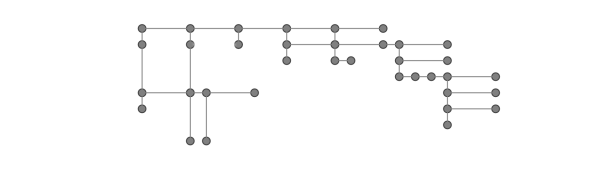
\includegraphics[width=0.8 \linewidth]{figure/nodeLink}
	\end{center}
	\caption{rappresentazione node-link HW drawing di un albero \label{fig:nodeLink}}
\end{figure}

Nella strategia Space-filling si tenta invece di superare i limiti del Node-link che riguardano la gestione non ottimale dello spazio orizzontale in quanto la parte alta della rappresentazione solitamente risulta essere poco densa di informazioni al contrario di quella bassa. Nella strategia Space-filling forme geometriche, solitamente rettangolari, rappresentano i nodi e i figli sono rappresentati da altre forme geometriche inserite all'interno del padre anche se anche questa rappresentazione presenta svariati problemi tra cui la distinzione difficile di tagli orizzontali da quelli verticali o la gestione non ottimale di alberi di grande profondità. Nella \textbf{\figurename~\ref{fig:spaceFilling}} sono mostrate alcune rappresentazioni diverse che seguono la strategia Space-filling.
\begin{figure}[!htb]
	\begin{center}
		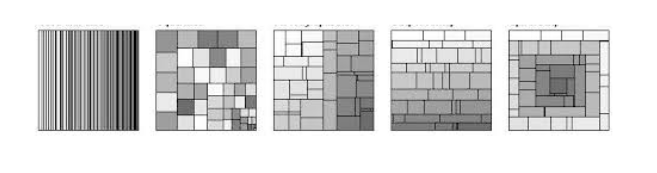
\includegraphics[width=0.9 \linewidth]{figure/spaceFilling}
	\end{center}
	\caption{rappresentazioni Space-filling\label{fig:spaceFilling}}
\end{figure}
\newline
Essendo quest'ultima di difficile lettura e soprattutto non ottimale per la rappresentazione di un albero collegato ad un grafo si consiglia di optare per la strategia Node-link scegliendo la rappresentazione "layered drawing",di cui ne è un esempio la \figurename{layered},in cui i nodi sono organizzati in livelli e per ogni nodo la coordinata y dipende dal livello mentre la coordinata x deve esser trovata e dipende dal numero di figli del livello e dello spazio orizzontale a disposizione per la rappresentazione.

\begin{figure}[!htb]
	\begin{center}
		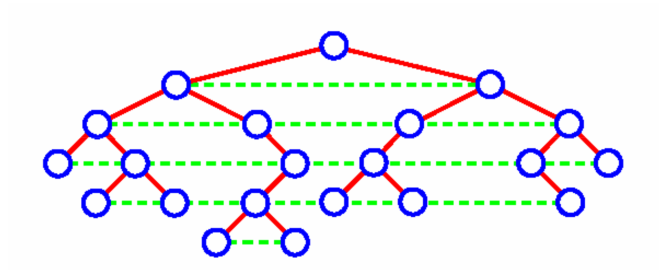
\includegraphics[width=0.9 \linewidth]{figure/layered}
	\end{center}
	\caption{rappresentazione node-Link layered Drawing\label{fig:layered}}
\end{figure}
\section{rappresentazione underlying Graph}
Avendo discusso della rappresentazione dell'inclusion Tree è necessaria la stessa attenzione per la rappresentazione dell'Underlying graph.  Essendo un albero un grafo orientato senza cicli i modelli di rappresentazione sono gli stessi visti per gli alberi. Il modello utilizzato è il \textbf{Force directed}, modello principale utilizzato per la visualizzazione di grafi che utilizza una rappresentazione Node-link, che fa in modo di emulare il sistema fisico formato da cariche elettriche rappresentate dai nodi e da molle rappresentati dagli archi. L'idea alla base del modello è quella che il raggiungimento di una condizione di equilibro corrisponda ad una rappresentazione grafica gradevole. ogni rappresentazione di un grafo è dunque formata da due componenti: il \textbf{modello} che descrive le forze in gioco e l'\textbf{algoritmo} ovvero la tecnica che permette di stabilire il punto di equilibrio accettabile. Ne esistono diverse varianti del modello Force directed e la scelta per quanto concerne il progetto in questone è ricaduta sul modello Spring Embedding, basato sulla combinazione di forze elettriche e forze meccaniche che andrà a formare una rappresentazione simile a quella mostrata nella \textbf{\figurename~\ref{fig:spring}}   
\begin{figure}[!htb]
	\begin{center}
		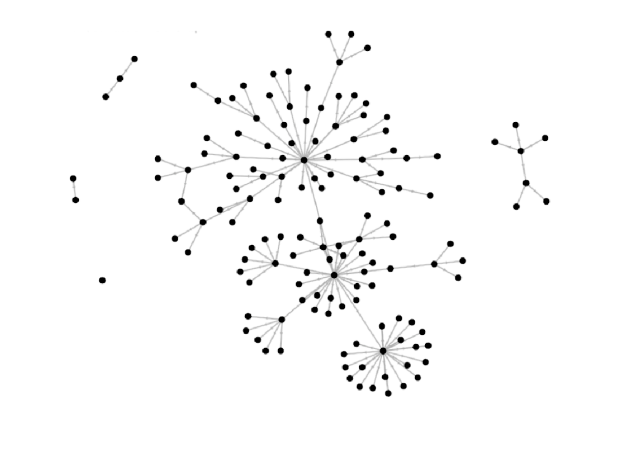
\includegraphics[width=0.8 \linewidth]{figure/spring}
	\end{center}
	\caption{rappresentazione Spring Embedding\label{fig:spring}}
\end{figure}
Per quanto concerne invece la complessità computazionale, il metodo non garantisce il numero di iterazione minimo per poter raggiungere una configurazione di equilibrio ed ogni passo iterativo ha complessità quadratica per i nodi e lineare per tutte le iterazioni avendo quindi un costo complessivo finale $O(n^3)$ senza lasciare però nessuna garanzia sul layout del grafo rappresentato.

}
